\documentclass[addpoints]{exam}
\usepackage[utf8]{inputenc}
\usepackage{multicol}
\usepackage{graphicx}
\usepackage{amsmath}
\usepackage{subcaption}
\usepackage[a4paper,top=15mm, bottom=15mm, left=15mm, right=15mm]{geometry}

%\printanswers

\newcommand{\tf}[1][{}]{%
	\fillin[#1][0.25in]%
}
 
\begin{document}
 
\begin{center}
	\fbox{\fbox{\parbox{5.5in}{\centering Istituti Card. C. Baronio - Vicenza \\ Anno scolastico 2019/2020 \\ Compito di Elettrotecnica - 3a TL}}}
\end{center}

\vspace{5mm}

\makebox[\textwidth]{Nome e Cognome:\enspace\hrulefill Data:\enspace\hrulefill}
 
\vspace{10mm}



\begin{questions}

\question[1] Date due cariche Q1=5C e Q2=10C, poste ad una distanza di 3cm l’una dall’altra, calcolare la loro forza di interazione. Calcolare poi il campo elettrico prodotto sulla carica Q2.

\question[1] Su un condensatore è presente una carica di 20C ed esso ha una capacità di 40mA, calcolare la tensione che è presente ai suoi capi e la sua energia immagazzinata.

\question[2] In un circuito circola una corrente di 3A quando viene applicata una tensione di 10V. Calcola la resistenza del circuito e la potenza che consuma. Se questa potenza viene consumata in 3 secondi, qual è la quantità di carica che è stata spostata?

\question[2] Sapendo che R1 = 3k$\Omega$, R2 = 5K$\Omega$, R3 = 2k$\Omega$ e R4 = 4k$\Omega$, calcola la resistenza equivalente del circuito Easy

\question[2] Sapendo che $C_1=5F, C_2=10F, C_3=7F, C_4=2F, C_5=4F$, calcola la capacità equivalente del circuito Medium

\question[2] Sapendo che $R_1=3k \Omega, R_2=5k \Omega, R3=2k \Omega, R_4=4k \Omega, R_5=3k \Omega, R_6=12k \Omega, R7=10k \Omega$, calcola la resistenza equivalente del circuito Hard

\end{questions}

\begin{figure}[h]
\begin{subfigure}{.5\textwidth}
  \centering
  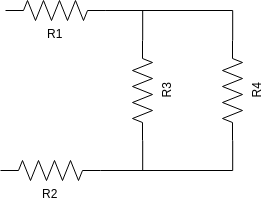
\includegraphics[width=0.8\linewidth]{ResistenzeEasy.png}
  \caption{Easy}
  \label{fig:sfig1}
\end{subfigure}%
\begin{subfigure}{.5\textwidth}
  \centering
  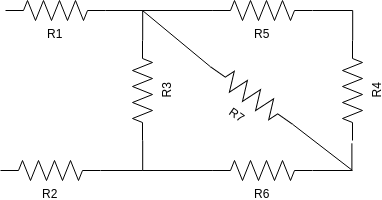
\includegraphics[width=1\linewidth]{ResistenzeHard.png}
  \caption{Hard}
  \label{fig:sfig2}
\end{subfigure}
\begin{subfigure}{.5\textwidth}
  \centering
  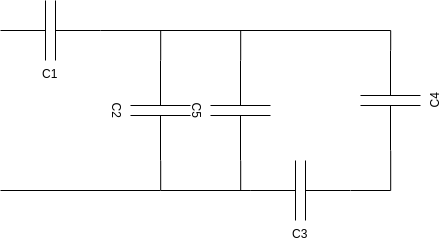
\includegraphics[width=1\linewidth]{CondensatoriMedium.png}
  \caption{Medium}
  \label{fig:sfig3}
\end{subfigure}
\begin{subfigure}{.5\textwidth}
  \centering
  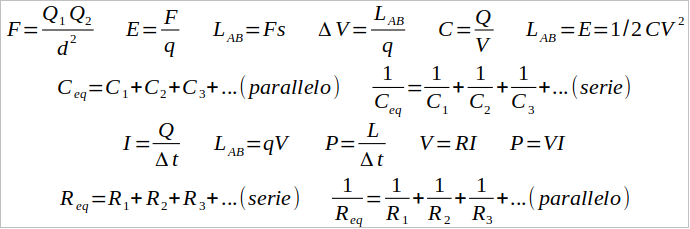
\includegraphics[width=1\linewidth]{Formulario.png}
  \caption{Formule}
  \label{fig:sfig3}
\end{subfigure}
\end{figure}

\begin{center}
	\gradetable[h][questions]
\end{center}




\end{document}